To evaluate the performance of the Monocular View Volume Registration (MVVR) method, both qualitative and quantitative types of experiment results are presented. In these experiments, the MVVR method was compared against the proposed FVR method. In some experiments, the Microsoft Life-Cam HD3000 passive camera was used capturing $640 \times 480$ images. In some comparisons, the ASUS Xtion PRO LIVE camera was used, but the MVVR method only made use of the information from the RGB frames. These images were processed and successive frames were used to generate depth maps. Each depth map was projected into volume sizes of $256^3$ for processing by the rest of the MVVR method (namely the FVR part). To generate the depth maps, a local 2D block matching method was used. Kernel sizes used in the correlation procedure were $3 \times 3$ in size with a search area size of $21 \times 21$. The sizes of the kernel, search area and volume sizes were all chosen empirically. \\


For the qualitative comparison, RGB-D frames of two scenes were captured using the ASUS Xtion PRO LIVE active camera, RGB-D information was fed into the FVR registration method whilst only RGB monocular data was fed into the MVVR algorithm. Figure \ref{fig:clockMVVRQResults} shows the qualitative comparison between the reconstruction generated via the FVR method (left) with the MVVR method (right) using the clock video stream. This video stream was captured by translating and rotating the camera slowly between frames. The depth maps computed by the block matching method are only an estimation of the true scene depth and therefore the projection is only relative to the
actual depth. However the 3D data in the registration is still spatially accurate relative to the different parts of the geometry within the scene. Comparing the noise levels between depth maps produced by block matching and RGB-D hardware (figure \ref{fig:DepthGenerationExample}) we can see how much more noise the MVVR method must tolerate in order to generate a 3D reconstruction. \\


\begin{figure}[!htb]
        \centering
        \begin{subfigure}[b]{1.8in}
                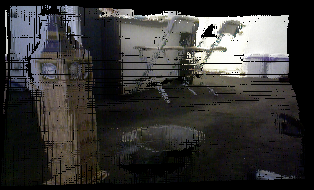
\includegraphics[width=1.5in]{images/results/mvvr/clockFVR}
                \label{fig:clockFVRRes}
        \end{subfigure}%
        \begin{subfigure}[b]{1.8in}
                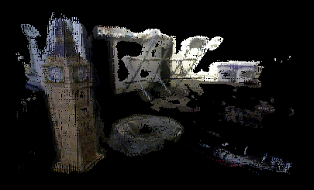
\includegraphics[width=1.5in]{images/results/mvvr/clockMVVR}
                \label{fig:clockMVVRRes}
        \end{subfigure}
        \caption{Registration of the Clock video stream using the FVR method (left) and the MVVR method (right).}
       \label{fig:clockMVVRQResults}
\end{figure}

Figure \ref{fig:boxesMVVRQResults} shows results from a similar qualitative experiment, this time using the boxes video stream. As with the qualitative experiment data in the clock scene, this stream was captured by moving the camera over the scene so that the environment is scanned in. The MVVR algorithm is again able to generate a dense 3D reconstructed model of the environment using only the noisy depth data computed via a monocular depth estimation procedure based on block matching. Parts of the scene which contain continuous texture are not and cannot (for the most part) be computed via this depth estimation procedure. Therefore, noticeable gaps are present in the output 3D reconstruction. \\



\begin{figure}[!htb]
        \centering
        \begin{subfigure}[b]{1.8in}
                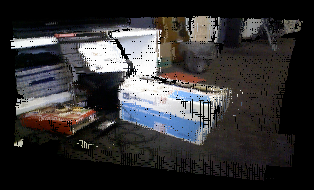
\includegraphics[width=1.5in]{images/results/mvvr/boxesFVR}
                \label{fig:boxFVRRes}
        \end{subfigure}%
        \begin{subfigure}[b]{1.8in}
                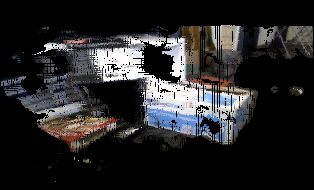
\includegraphics[width=1.5in]{images/results/mvvr/boxesMVVR}
                \label{fig:boxMVVRRes}
        \end{subfigure}
        \caption{Registration of the Boxes video stream using the FVR method (left) and the MVVR method (right).}
       \label{fig:boxesMVVRQResults}
\end{figure}

Qualitative results show that with qualitative performance which approaches that of the FVR (the higher the quality of the depth map produced) and without performing any feature matching, the MVVR method is able to register dense depth data and produce results comparable to the FVR registration method despite the noise prevalent in the block matching depth estimates. \\

In order to assess the method quantitatively, frames were captured using the Microsoft LifeCam HD3000 passive camera was moved in 5 centimeter, 10 centimeter and 15 centimeter increments. Depth maps were again produced via 2D block matching, these depth maps were then projected and registered using the FVR method to compute the camera movement between frames. These estimated camera movements were then compared to ground truth recordings. Results are placed in table \ref{table:transMVVR}.

%translation
\begin{table}[!htb]
\centering
\scalebox{1.0}{
\begin{tabular}{ccc}
\hline
\textbf{movement (cm)} & \textbf{FVR-Error} & \textbf{MVVR-Error}\\ \hline
5cm &  0 & 0\\
10cm & 0 & 0\\
15cm & 0 & 27cm\\
\\
\end{tabular}}
\\
\caption{Translation Tracking Error for FVR and MVVR}
\label{table:transMVVR}
\end{table}


Table \ref{table:transMVVR} shows that in these experiments, the RGB-D VR method was able to register with 100\% accuracy camera movements with up to 15 centimeters of camera movement between frames. With the same data, the MVVR method is capable of registering the camera movement despite the requirement of tolerating inconsistent and noisy depth information. The MVVR method is shown to be able to register up to 10 centimeters of camera movement without fault. With movements of 10 centimeters and frame rates of 30 frames per second, this equates to speeds of roughly 10 kilo-meters per hour. This is about twice the average walking speed of a person. \\

